\documentclass{standalone}
\usepackage{tikz}
\usetikzlibrary{patterns, positioning}


\begin{document}
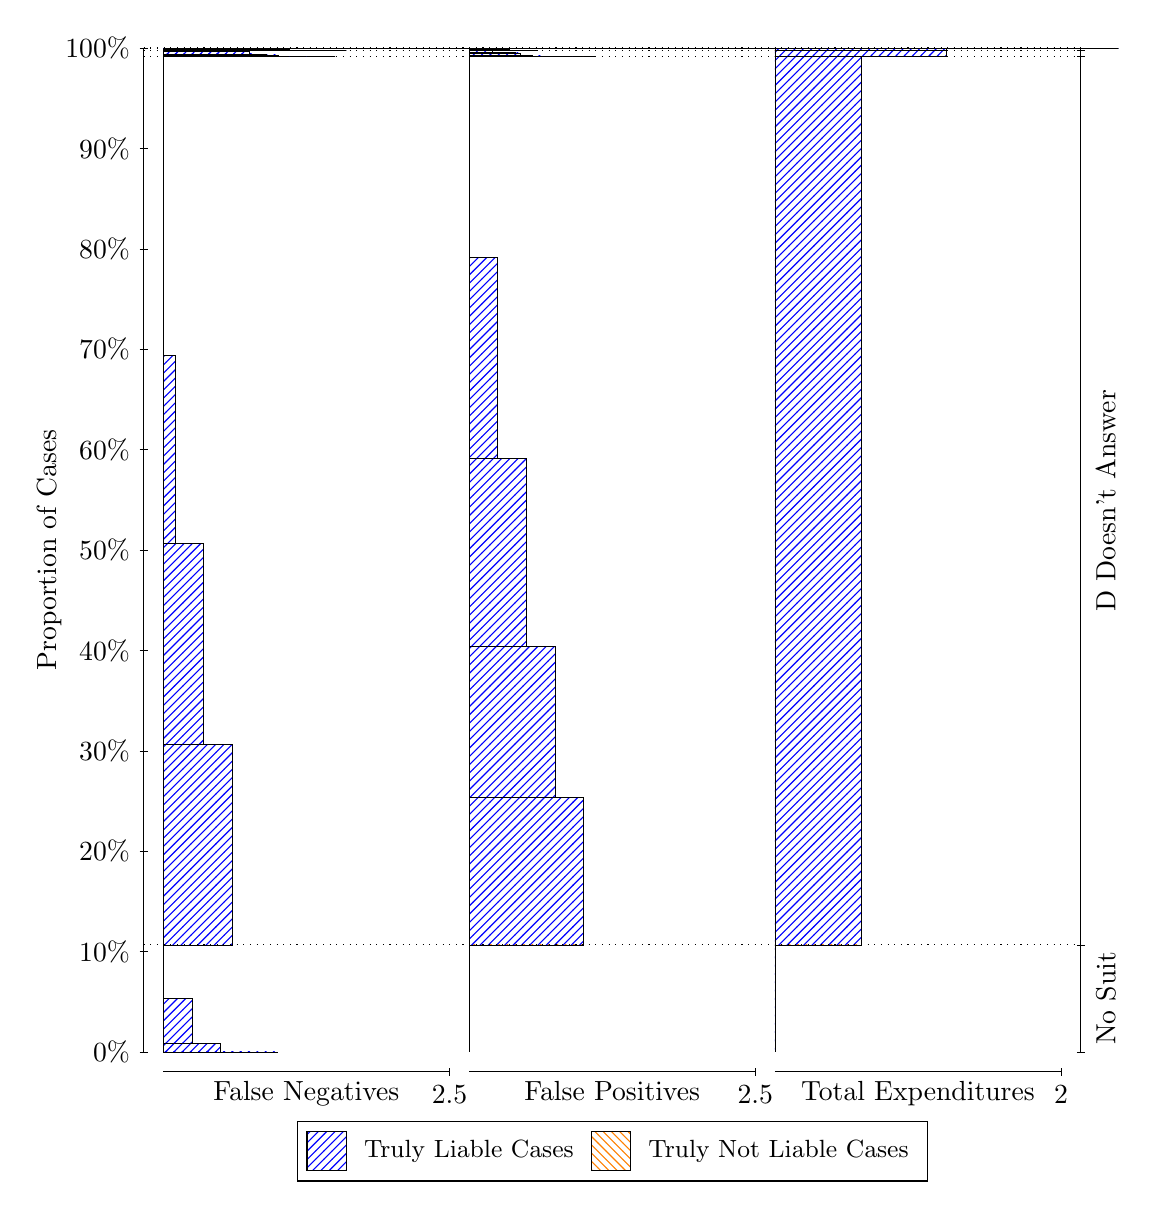
\begin{tikzpicture}
\draw[black, very thin] (1.5,1.75) -- (1.5,14.5);
\node[rotate=90, text=black, anchor=center] at (0.3, 8.125) {Proportion of Cases};
\draw[black, very thin] (1.45,1.75) -- (1.55,1.75);
\node[text=black, anchor=east] at (1.45, 1.75) {0\%};
\draw[black, very thin] (1.45,3.025) -- (1.55,3.025);
\node[text=black, anchor=east] at (1.45, 3.025) {10\%};
\draw[black, very thin] (1.45,4.3) -- (1.55,4.3);
\node[text=black, anchor=east] at (1.45, 4.3) {20\%};
\draw[black, very thin] (1.45,5.575) -- (1.55,5.575);
\node[text=black, anchor=east] at (1.45, 5.575) {30\%};
\draw[black, very thin] (1.45,6.85) -- (1.55,6.85);
\node[text=black, anchor=east] at (1.45, 6.85) {40\%};
\draw[black, very thin] (1.45,8.125) -- (1.55,8.125);
\node[text=black, anchor=east] at (1.45, 8.125) {50\%};
\draw[black, very thin] (1.45,9.4) -- (1.55,9.4);
\node[text=black, anchor=east] at (1.45, 9.4) {60\%};
\draw[black, very thin] (1.45,10.675) -- (1.55,10.675);
\node[text=black, anchor=east] at (1.45, 10.675) {70\%};
\draw[black, very thin] (1.45,11.95) -- (1.55,11.95);
\node[text=black, anchor=east] at (1.45, 11.95) {80\%};
\draw[black, very thin] (1.45,13.225) -- (1.55,13.225);
\node[text=black, anchor=east] at (1.45, 13.225) {90\%};
\draw[black, very thin] (1.45,14.5) -- (1.55,14.5);
\node[text=black, anchor=east] at (1.45, 14.5) {100\%};

\draw[black, very thin] (13.4,1.75) -- (13.4,14.5);
\draw[black, very thin] (13.35,1.75) -- (13.45,1.75);
\node[anchor=west] at (13.35, 1.75) {};
\draw[black, very thin] (13.35,3.1097) -- (13.45,3.1097);
\node[anchor=west] at (13.35, 3.1097) {};
\draw[black, very thin] (13.35,14.39) -- (13.45,14.39);
\node[anchor=west] at (13.35, 14.39) {};
\draw[black, very thin] (13.35,14.472) -- (13.45,14.472);
\node[anchor=west] at (13.35, 14.472) {};
\draw[black, very thin] (13.35,14.494) -- (13.45,14.494);
\node[anchor=west] at (13.35, 14.494) {};
\draw[black, very thin] (13.35,14.5) -- (13.45,14.5);
\node[anchor=west] at (13.35, 14.5) {};
\draw[black, very thin] (13.35,14.5) -- (13.45,14.5);
\node[anchor=west] at (13.35, 14.5) {};

\draw[black, very thin, pattern color=blue, pattern=north east lines] (1.75,1.75) rectangle (3.2033,1.75);
\draw[black, very thin, pattern color=blue, pattern=north east lines] (1.75,1.75) rectangle (2.84,1.7509);
\draw[black, very thin, pattern color=blue, pattern=north east lines] (1.75,1.7509) rectangle (2.4767,1.8588);
\draw[black, very thin, pattern color=blue, pattern=north east lines] (1.75,1.8588) rectangle (2.1133,2.4308);
\draw[black, very thin, pattern color=orange, pattern=north west lines] (1.75,2.4308) rectangle (1.75,2.4308);
\draw[black, very thin, pattern color=blue, pattern=north east lines] (1.75,2.4308) rectangle (1.75,3.1097);
\draw[black, very thin, pattern color=blue, pattern=north east lines] (1.75,3.1097) rectangle (2.622,5.6596);
\draw[black, very thin, pattern color=blue, pattern=north east lines] (1.75,5.6596) rectangle (2.2587,8.2082);
\draw[black, very thin, pattern color=blue, pattern=north east lines] (1.75,8.2082) rectangle (1.8953,10.6);
\draw[black, very thin, pattern color=orange, pattern=north west lines] (1.75,10.6) rectangle (1.75,10.6);
\draw[black, very thin, pattern color=blue, pattern=north east lines] (1.75,10.6) rectangle (1.75,14.39);
\draw[black, very thin, pattern color=blue, pattern=north east lines] (1.75,14.39) rectangle (3.93,14.39);
\draw[black, very thin, pattern color=blue, pattern=north east lines] (1.75,14.39) rectangle (3.7847,14.39);
\draw[black, very thin, pattern color=blue, pattern=north east lines] (1.75,14.39) rectangle (3.6393,14.39);
\draw[black, very thin, pattern color=blue, pattern=north east lines] (1.75,14.39) rectangle (3.5667,14.39);
\draw[black, very thin, pattern color=blue, pattern=north east lines] (1.75,14.39) rectangle (3.494,14.39);
\draw[black, very thin, pattern color=blue, pattern=north east lines] (1.75,14.39) rectangle (3.4213,14.39);
\draw[black, very thin, pattern color=blue, pattern=north east lines] (1.75,14.39) rectangle (3.3487,14.39);
\draw[black, very thin, pattern color=blue, pattern=north east lines] (1.75,14.39) rectangle (3.276,14.39);
\draw[black, very thin, pattern color=blue, pattern=north east lines] (1.75,14.39) rectangle (3.2033,14.414);
\draw[black, very thin, pattern color=blue, pattern=north east lines] (1.75,14.414) rectangle (3.1307,14.414);
\draw[black, very thin, pattern color=blue, pattern=north east lines] (1.75,14.414) rectangle (3.058,14.418);
\draw[black, very thin, pattern color=blue, pattern=north east lines] (1.75,14.418) rectangle (2.9853,14.418);
\draw[black, very thin, pattern color=blue, pattern=north east lines] (1.75,14.418) rectangle (2.9127,14.425);
\draw[black, very thin, pattern color=blue, pattern=north east lines] (1.75,14.425) rectangle (2.84,14.456);
\draw[black, very thin, pattern color=blue, pattern=north east lines] (1.75,14.456) rectangle (2.7673,14.457);
\draw[black, very thin, pattern color=blue, pattern=north east lines] (1.75,14.457) rectangle (2.6947,14.461);
\draw[black, very thin, pattern color=blue, pattern=north east lines] (1.75,14.461) rectangle (2.622,14.462);
\draw[black, very thin, pattern color=blue, pattern=north east lines] (1.75,14.462) rectangle (2.5493,14.47);
\draw[black, very thin, pattern color=blue, pattern=north east lines] (1.75,14.47) rectangle (2.4767,14.471);
\draw[black, very thin, pattern color=blue, pattern=north east lines] (1.75,14.471) rectangle (2.404,14.471);
\draw[black, very thin, pattern color=blue, pattern=north east lines] (1.75,14.471) rectangle (2.3313,14.471);
\draw[black, very thin, pattern color=blue, pattern=north east lines] (1.75,14.471) rectangle (2.2587,14.471);
\draw[black, very thin, pattern color=blue, pattern=north east lines] (1.75,14.471) rectangle (2.186,14.472);
\draw[black, very thin, pattern color=blue, pattern=north east lines] (1.75,14.472) rectangle (2.0407,14.472);
\draw[black, very thin, pattern color=blue, pattern=north east lines] (1.75,14.472) rectangle (1.8953,14.472);
\draw[black, very thin, pattern color=orange, pattern=north west lines] (1.75,14.472) rectangle (1.75,14.472);
\draw[black, very thin, pattern color=blue, pattern=north east lines] (1.75,14.472) rectangle (4.0753,14.472);
\draw[black, very thin, pattern color=blue, pattern=north east lines] (1.75,14.472) rectangle (3.712,14.472);
\draw[black, very thin, pattern color=blue, pattern=north east lines] (1.75,14.472) rectangle (3.3487,14.482);
\draw[black, very thin, pattern color=blue, pattern=north east lines] (1.75,14.482) rectangle (2.9853,14.494);
\draw[black, very thin, pattern color=blue, pattern=north east lines] (1.75,14.494) rectangle (2.622,14.494);
\draw[black, very thin, pattern color=orange, pattern=north west lines] (1.75,14.494) rectangle (1.75,14.494);
\draw[black, very thin, pattern color=blue, pattern=north east lines] (1.75,14.494) rectangle (2.622,14.494);
\draw[black, very thin, pattern color=blue, pattern=north east lines] (1.75,14.494) rectangle (2.2587,14.494);
\draw[black, very thin, pattern color=blue, pattern=north east lines] (1.75,14.494) rectangle (1.8953,14.498);
\draw[black, very thin, pattern color=orange, pattern=north west lines] (1.75,14.498) rectangle (1.75,14.498);
\draw[black, very thin, pattern color=blue, pattern=north east lines] (1.75,14.498) rectangle (1.75,14.5);
\draw[black, very thin, pattern color=blue, pattern=north east lines] (1.75,14.5) rectangle (6.6913,14.5);
\draw[black, very thin, pattern color=blue, pattern=north east lines] (1.75,14.5) rectangle (6.328,14.5);
\draw[black, very thin, pattern color=blue, pattern=north east lines] (1.75,14.5) rectangle (5.9647,14.5);
\draw[black, very thin, pattern color=blue, pattern=north east lines] (1.75,14.5) rectangle (5.6013,14.5);
\draw[black, very thin, pattern color=blue, pattern=north east lines] (1.75,14.5) rectangle (5.238,14.5);
\draw[black, very thin, pattern color=blue, pattern=north east lines] (1.75,14.5) rectangle (4.8747,14.5);
\draw[black, very thin, pattern color=blue, pattern=north east lines] (1.75,14.5) rectangle (2.84,14.5);
\draw[black, very thin, pattern color=blue, pattern=north east lines] (1.75,14.5) rectangle (2.4767,14.5);
\draw[black, very thin, pattern color=blue, pattern=north east lines] (1.75,14.5) rectangle (2.1133,14.5);
\draw[black, very thin, pattern color=orange, pattern=north west lines] (1.75,14.5) rectangle (1.75,14.5);
\draw[black, very thin, pattern color=blue, pattern=north east lines] (1.75,14.5) rectangle (1.75,14.5);
\draw[black, very thin, pattern color=orange, pattern=north west lines] (5.6333,1.75) rectangle (5.6333,1.75);
\draw[black, very thin, pattern color=blue, pattern=north east lines] (5.6333,1.75) rectangle (5.6333,3.1097);
\draw[black, very thin, pattern color=orange, pattern=north west lines] (5.6333,3.1097) rectangle (7.0867,3.1097);
\draw[black, very thin, pattern color=blue, pattern=north east lines] (5.6333,3.1097) rectangle (7.0867,4.9798);
\draw[black, very thin, pattern color=blue, pattern=north east lines] (5.6333,4.9798) rectangle (6.7233,6.9001);
\draw[black, very thin, pattern color=blue, pattern=north east lines] (5.6333,6.9001) rectangle (6.36,9.2918);
\draw[black, very thin, pattern color=blue, pattern=north east lines] (5.6333,9.2918) rectangle (5.9967,11.84);
\draw[black, very thin, pattern color=blue, pattern=north east lines] (5.6333,11.84) rectangle (5.6333,14.39);
\draw[black, very thin, pattern color=orange, pattern=north west lines] (5.6333,14.39) rectangle (7.232,14.39);
\draw[black, very thin, pattern color=blue, pattern=north east lines] (5.6333,14.39) rectangle (7.232,14.39);
\draw[black, very thin, pattern color=orange, pattern=north west lines] (5.6333,14.39) rectangle (7.0867,14.39);
\draw[black, very thin, pattern color=blue, pattern=north east lines] (5.6333,14.39) rectangle (7.0867,14.39);
\draw[black, very thin, pattern color=orange, pattern=north west lines] (5.6333,14.39) rectangle (6.9413,14.39);
\draw[black, very thin, pattern color=blue, pattern=north east lines] (5.6333,14.39) rectangle (6.9413,14.39);
\draw[black, very thin, pattern color=blue, pattern=north east lines] (5.6333,14.39) rectangle (6.8687,14.391);
\draw[black, very thin, pattern color=orange, pattern=north west lines] (5.6333,14.391) rectangle (6.796,14.391);
\draw[black, very thin, pattern color=blue, pattern=north east lines] (5.6333,14.391) rectangle (6.796,14.391);
\draw[black, very thin, pattern color=blue, pattern=north east lines] (5.6333,14.391) rectangle (6.7233,14.391);
\draw[black, very thin, pattern color=orange, pattern=north west lines] (5.6333,14.391) rectangle (6.6507,14.391);
\draw[black, very thin, pattern color=blue, pattern=north east lines] (5.6333,14.391) rectangle (6.6507,14.392);
\draw[black, very thin, pattern color=blue, pattern=north east lines] (5.6333,14.392) rectangle (6.578,14.4);
\draw[black, very thin, pattern color=blue, pattern=north east lines] (5.6333,14.4) rectangle (6.5053,14.401);
\draw[black, very thin, pattern color=blue, pattern=north east lines] (5.6333,14.401) rectangle (6.4327,14.405);
\draw[black, very thin, pattern color=blue, pattern=north east lines] (5.6333,14.405) rectangle (6.36,14.406);
\draw[black, very thin, pattern color=blue, pattern=north east lines] (5.6333,14.406) rectangle (6.2873,14.437);
\draw[black, very thin, pattern color=blue, pattern=north east lines] (5.6333,14.437) rectangle (6.2147,14.444);
\draw[black, very thin, pattern color=blue, pattern=north east lines] (5.6333,14.444) rectangle (6.142,14.444);
\draw[black, very thin, pattern color=blue, pattern=north east lines] (5.6333,14.444) rectangle (6.0693,14.448);
\draw[black, very thin, pattern color=blue, pattern=north east lines] (5.6333,14.448) rectangle (5.9967,14.448);
\draw[black, very thin, pattern color=blue, pattern=north east lines] (5.6333,14.448) rectangle (5.924,14.472);
\draw[black, very thin, pattern color=blue, pattern=north east lines] (5.6333,14.472) rectangle (5.8513,14.472);
\draw[black, very thin, pattern color=blue, pattern=north east lines] (5.6333,14.472) rectangle (5.7787,14.472);
\draw[black, very thin, pattern color=blue, pattern=north east lines] (5.6333,14.472) rectangle (5.706,14.472);
\draw[black, very thin, pattern color=blue, pattern=north east lines] (5.6333,14.472) rectangle (5.6333,14.472);
\draw[black, very thin, pattern color=orange, pattern=north west lines] (5.6333,14.472) rectangle (6.5053,14.472);
\draw[black, very thin, pattern color=blue, pattern=north east lines] (5.6333,14.472) rectangle (6.5053,14.472);
\draw[black, very thin, pattern color=blue, pattern=north east lines] (5.6333,14.472) rectangle (6.142,14.484);
\draw[black, very thin, pattern color=blue, pattern=north east lines] (5.6333,14.484) rectangle (5.7787,14.494);
\draw[black, very thin, pattern color=blue, pattern=north east lines] (5.6333,14.494) rectangle (5.6333,14.494);
\draw[black, very thin, pattern color=orange, pattern=north west lines] (5.6333,14.494) rectangle (7.9587,14.494);
\draw[black, very thin, pattern color=blue, pattern=north east lines] (5.6333,14.494) rectangle (7.9587,14.494);
\draw[black, very thin, pattern color=blue, pattern=north east lines] (5.6333,14.494) rectangle (7.5953,14.496);
\draw[black, very thin, pattern color=blue, pattern=north east lines] (5.6333,14.496) rectangle (7.232,14.499);
\draw[black, very thin, pattern color=blue, pattern=north east lines] (5.6333,14.499) rectangle (6.8687,14.5);
\draw[black, very thin, pattern color=blue, pattern=north east lines] (5.6333,14.5) rectangle (6.5053,14.5);
\draw[black, very thin, pattern color=orange, pattern=north west lines] (5.6333,14.5) rectangle (10.575,14.5);
\draw[black, very thin, pattern color=blue, pattern=north east lines] (5.6333,14.5) rectangle (10.575,14.5);
\draw[black, very thin, pattern color=orange, pattern=north west lines] (5.6333,14.5) rectangle (10.211,14.5);
\draw[black, very thin, pattern color=blue, pattern=north east lines] (5.6333,14.5) rectangle (10.211,14.5);
\draw[black, very thin, pattern color=orange, pattern=north west lines] (5.6333,14.5) rectangle (9.848,14.5);
\draw[black, very thin, pattern color=blue, pattern=north east lines] (5.6333,14.5) rectangle (9.848,14.5);
\draw[black, very thin, pattern color=orange, pattern=north west lines] (5.6333,14.5) rectangle (9.4847,14.5);
\draw[black, very thin, pattern color=blue, pattern=north east lines] (5.6333,14.5) rectangle (9.4847,14.5);
\draw[black, very thin, pattern color=blue, pattern=north east lines] (5.6333,14.5) rectangle (9.1213,14.5);
\draw[black, very thin, pattern color=blue, pattern=north east lines] (5.6333,14.5) rectangle (8.758,14.5);
\draw[black, very thin, pattern color=blue, pattern=north east lines] (5.6333,14.5) rectangle (8.3947,14.5);
\draw[black, very thin, pattern color=blue, pattern=north east lines] (5.6333,14.5) rectangle (8.0313,14.5);
\draw[black, very thin, pattern color=orange, pattern=north west lines] (5.6333,14.5) rectangle (5.9967,14.5);
\draw[black, very thin, pattern color=blue, pattern=north east lines] (5.6333,14.5) rectangle (5.9967,14.5);
\draw[black, very thin, pattern color=orange, pattern=north west lines] (5.6333,14.5) rectangle (5.6333,14.5);
\draw[black, very thin, pattern color=blue, pattern=north east lines] (5.6333,14.5) rectangle (5.6333,14.5);
\draw[black, very thin, pattern color=orange, pattern=north west lines] (9.5167,1.75) rectangle (9.5167,1.75);
\draw[black, very thin, pattern color=blue, pattern=north east lines] (9.5167,1.75) rectangle (9.5167,3.1097);
\draw[black, very thin, pattern color=orange, pattern=north west lines] (9.5167,3.1097) rectangle (10.607,3.1097);
\draw[black, very thin, pattern color=blue, pattern=north east lines] (9.5167,3.1097) rectangle (10.607,14.39);
\draw[black, very thin, pattern color=orange, pattern=north west lines] (9.5167,14.39) rectangle (11.697,14.39);
\draw[black, very thin, pattern color=blue, pattern=north east lines] (9.5167,14.39) rectangle (11.697,14.392);
\draw[black, very thin, pattern color=orange, pattern=north west lines] (9.5167,14.392) rectangle (11.697,14.392);
\draw[black, very thin, pattern color=blue, pattern=north east lines] (9.5167,14.392) rectangle (11.697,14.472);
\draw[black, very thin, pattern color=orange, pattern=north west lines] (9.5167,14.472) rectangle (11.697,14.472);
\draw[black, very thin, pattern color=blue, pattern=north east lines] (9.5167,14.472) rectangle (11.697,14.494);
\draw[black, very thin, pattern color=orange, pattern=north west lines] (9.5167,14.494) rectangle (11.697,14.494);
\draw[black, very thin, pattern color=blue, pattern=north east lines] (9.5167,14.494) rectangle (11.697,14.5);
\draw[black, very thin, pattern color=orange, pattern=north west lines] (9.5167,14.5) rectangle (13.877,14.5);
\draw[black, very thin, pattern color=blue, pattern=north east lines] (9.5167,14.5) rectangle (13.877,14.5);
\draw[black, dotted] (1.5,3.1097) -- (13.4,3.1097);
\draw[black, dotted] (1.5,14.39) -- (13.4,14.39);
\draw[black, dotted] (1.5,14.472) -- (13.4,14.472);
\draw[black, dotted] (1.5,14.494) -- (13.4,14.494);
\draw[black, dotted] (1.5,14.5) -- (13.4,14.5);
\draw[black, very thin] (1.75,1.5) -- (5.3833,1.5);
\node[text=black, anchor=north] at (3.5667, 1.5) {False Negatives};
\draw[black, very thin] (5.3833,1.45) -- (5.3833,1.55);
\node[text=black, anchor=north] at (5.3833, 1.45) {2.5};

\draw[black, very thin] (5.6333,1.5) -- (9.2667,1.5);
\node[text=black, anchor=north] at (7.45, 1.5) {False Positives};
\draw[black, very thin] (9.2667,1.45) -- (9.2667,1.55);
\node[text=black, anchor=north] at (9.2667, 1.45) {2.5};

\draw[black, very thin] (9.5167,1.5) -- (13.15,1.5);
\node[text=black, anchor=north] at (11.333, 1.5) {Total Expenditures};
\draw[black, very thin] (13.15,1.45) -- (13.15,1.55);
\node[text=black, anchor=north] at (13.15, 1.45) {2};

\node[text=black, centered, rotate=90] at (13.72, 2.4298) {No Suit};
\node[text=black, centered, rotate=90] at (13.72, 8.75) {D Doesn't Answer};





\draw (7.449999999999999,1.5) node[draw=none] (baseCoordinate) {};
\begin{scope}[align=center]
        \matrix[scale=0.5, draw=black, below=0.5cm of baseCoordinate, nodes={draw}, column sep=0.1cm]{
            \node[rectangle, draw, minimum width=0.5cm, minimum height=0.5cm, pattern color=blue, pattern=north east lines] {}; &
            \node[draw=none, font=\small, text=black] (B) {Truly Liable Cases}; &
            \node[rectangle, draw, minimum width=0.5cm, minimum height=0.5cm, pattern color=orange, pattern=north west lines] {}; &
            \node[draw=none, font=\small, text=black] (B) {Truly Not Liable Cases}; \\
            };
\end{scope}

\end{tikzpicture}
\end{document}